\documentclass[10pt,landscape,a4paper]{article}
\usepackage[utf8]{inputenc}
\usepackage[ngerman]{babel}
\usepackage{PTSansNarrow} 
\renewcommand*\familydefault{\sfdefault} %% Only if the base font of the document is to be sans serif
\usepackage[T1]{fontenc}
\usepackage[dvipsnames]{xcolor}
\usepackage{colortbl}
\usepackage{multicol}
\usepackage{float}
\usepackage[top=0mm,bottom=1mm,left=0mm,right=1mm]{geometry}
\usepackage{microtype}
\usepackage{enumitem}
\usepackage{booktabs}
\usepackage{tikz}
\usetikzlibrary{arrows.meta,graphs,shapes.misc}
\usepackage{amssymb}
\usepackage{amsmath}

\setlength{\jot}{0pt}
\appto{\footnotesize}{
	\setlength{\abovedisplayskip}{0pt}
	\setlength{\belowdisplayskip}{0pt}
	\setlength{\abovedisplayshortskip}{0pt}
	\setlength{\belowdisplayshortskip}{0pt}
}

\newenvironment{Figure}
  {\par\medskip\noindent\minipage{\linewidth}}
  {\endminipage\par\medskip}

\pagestyle{empty}
\renewcommand{\baselinestretch}{0.9}

\makeatletter
\renewcommand{\section}{\@startsection{section}{1}{0mm}%
                                {.2ex}%
                                {.2ex}%x
								{\sffamily\small\bfseries}}
\renewcommand{\paragraph}{\@startsection{paragraph}{1}{0mm}%
                                {.2ex}%
                                {.2ex}%x
								{\sffamily\bfseries}*}
\newcommand*{\rsimdots}{%
  \mathrel{%
    \mathpalette\@rsimdots{}% Adopt to math style size via \mathpalette
  }%
}
\newcommand*{\@rsimdots}[2]{%
  % #1: math style
  % #2: unused
  \sbox0{$#1\sim\m@th$}%
  \sbox2{$#1\vcenter{}$}% \ht2 is height of the math axis
  \dimen@=.75\ht2\relax % distance dot to math axis
  \sbox2{$#1\cdot\m@th$}% single vertically centered dot
  \sbox2{% two dots above and below the math axis
    \rlap{\raisebox{\dimen@}{\copy2}}%
    \raisebox{-\dimen@}{\copy2}%
  }%
  % Rotate the two dots.
  \sbox2{$#1\rotatebox[origin=c]{-45}{\copy2}$}%
  % Combine symbol
  \rlap{\hbox to \wd0{\hss\copy2\hss}}%
  \copy0 %
}
\makeatother

\setlist[itemize]{noitemsep,nolistsep,leftmargin=*}
\setlist[enumerate]{noitemsep,nolistsep,leftmargin=*}
\setlength{\parindent}{0pt}

\begin{document}
\footnotesize
\begin{multicols*}{5}
	\section{Chapter 1: Introduction}
\centering
\paragraph{Sample}
Subset of population which we have data on\\
$\Downarrow$
\paragraph{Descriptive Statistics} 
Summary Statistics of Sample Data\\
$\Downarrow$\\
Used to make \textsl{Inferences}\\
$\Downarrow$
\paragraph{Inferential Statistics}
Parameters of Population\\
(Unknown)\\
$\Downarrow$
\paragraph{Population} 
Total set of subjects of interest\\
	\raggedright
\section{Chapter 2: Single Variable Analyses}
\paragraph{Types of Variables}
\centering
Nominal \makebox[0pt][l]{(Cate)}\\
\makebox[0pt][r]{Meaningful Order\ }$\Downarrow$\\
Ordinal \makebox[0pt][l]{(Cate)}\\
\makebox[0pt][r]{Consistent Difference\ }$\Downarrow$\\
Discrete \makebox[0pt][l]{(Quant)}\\
\makebox[0pt][r]{(Uncountably) Infinite\ }$\Downarrow$\\
Continuous \makebox[0pt][l]{(Quant)}

\raggedright
\paragraph{Describing Data}
\textcolor{Bittersweet}{Continuous Variables:}
\begin{itemize}
	\item Cluster/Gap Intervals
	\item Suspected Outliers [Small/Large] ($z-score>3$)
	\item Modality
	\item Skewness
	\begin{enumerate}
		\item Symmetric \& Bell-Shaped: (Sensitive to Skew)
		\begin{itemize}
			\item Mean
			\item Var \& Std Dev
		\end{itemize}
		\item Highly Skewed: (Robust to Outliers)
		\begin{itemize}
			\item Median
			\item IQR (NOTE: Quantiles are non-unique)
		\end{itemize}
	\end{enumerate}
\end{itemize}
$\Rightarrow$ Continuous can be categorised!\\
\textcolor{Bittersweet}{Categorical (or Discrete) Variables:}
\begin{itemize}
	\item \% Proportion of Modal Category
	\item Special High/Low Categories
	\item (Ordinal) Apparent Trend in Proportions
\end{itemize}
\paragraph{Formulae and Results}
$\overline{X}=\frac{1}{n}\sum_{i=1}^nX_i$\\
$Var(X)=\frac{1}{n-1}\sum_{i-1}^n(X_i-\overline{X})^2$\\
\textcolor{Blue}{For $Y=aX+b$:}\\
$\overline{Y}=a\overline{X}+b$\\
$Var(Y)=a^2Var(X)$\\
$s_Y=\left|a\right|s_X$
\begin{Figure}
	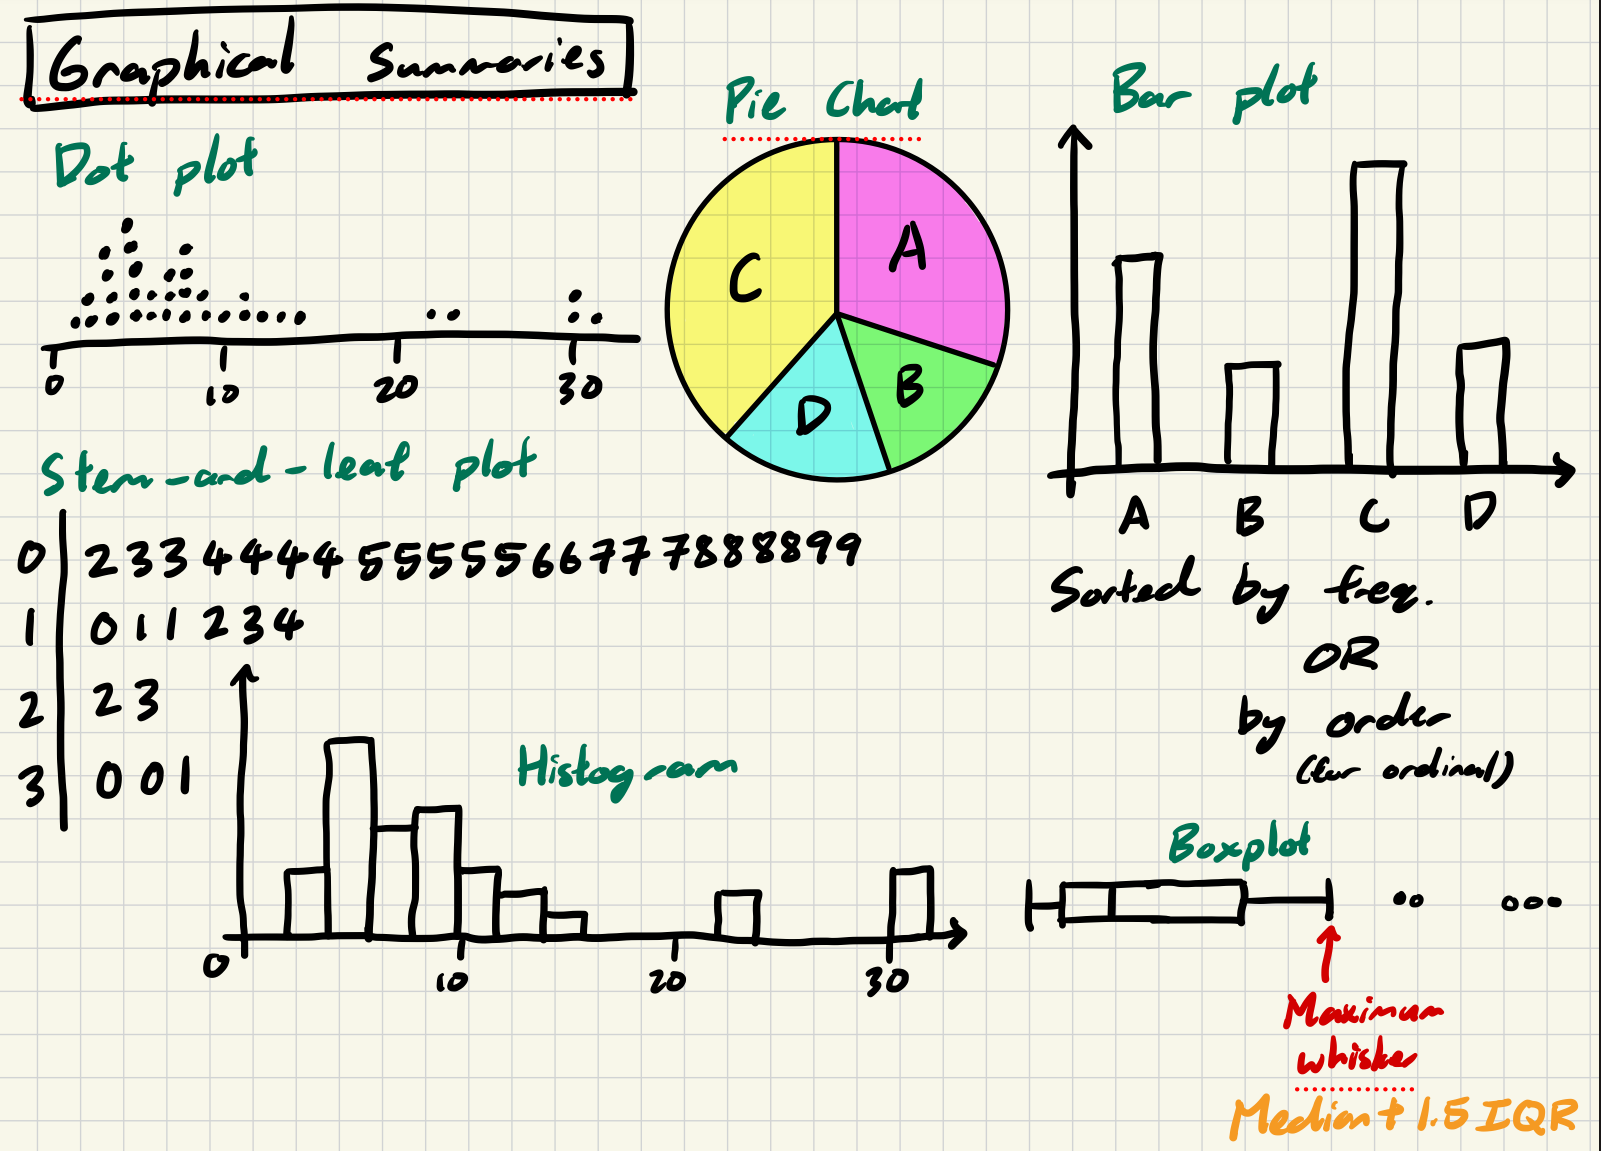
\includegraphics[width=\linewidth]{graphicalSummaries.png}
\end{Figure}
	\section{Association between Variables}
\paragraph{Categorical x Categorical}
\textcolor{Blue}{Association:}\\
\begin{itemize}
	\item Difference in Proportions
	\item Relative Risk $\frac{Occurrence\ in\ Exposed}{Occurrence\ in\ Unexposed}$
\end{itemize}
\textcolor{Blue}{Graphical Summaries:}
\begin{itemize}
	\item Contingency Table\\
		Conditional Proportions on [Explanatory] for [Response]\\
	 	Columns: Response, Rows: Explanatory\\
		$\sum$ proportions across row $=1$\\
		$Marginal\ Proportion=\frac{+\ Response}{Total\ Data}$
	\item Bar Charts (Stacked/Clustered)
\end{itemize}
\paragraph{Categorical x Quantitative}
\textcolor{Blue}{Association:}
\begin{itemize}
	\item Medians
	\item Skewness, Spread
	\item Outliers [Small/Large]
\end{itemize}
\textcolor{Blue}{Graphical Summary:} Side-by-side Boxplots
\paragraph{Quantitative x Quantitative}
\textcolor{Blue}{Association:}
\begin{itemize}
	\item Presence of Association [+/-]
	\item Type of Association [Linear/Non-Linear]
	\item Variance of Points
	\item Unusual Departure from Overall Trend\\
		\textcolor{Gray}{Non-Constant Variance, Suspected Outliers}
	\item Correlation Coefficient (Linear only)
		\[R=\frac{1}{n-1}\sum(\frac{X_i-\overline{X}}{s_X})(\frac{Y_i-\overline{Y}}{s_Y})\]\\
		Interpretation:\\
		\begin{center}
			\begin{tabular}{c c}
				\midrule
				$\left|R\right|>=0.8$ & Very Strong\\
				$0.5<\left|R\right|<0.8$ & Strong\\
				$\left|R\right|<=0.5$ & Not Strong\\
				\midrule
			\end{tabular}
		\end{center}
\end{itemize}
Correlation != Causation$\Downarrow$
\paragraph{Lurking and Confounding Variables}
\textcolor{Bittersweet}{Lurking Variables}: Unobserved variable that influences association between
variables of interest. Has potential for confounding.\\
\textcolor{Bittersweet}{Confounding Variables}: Explanatory variables which are associated with response,
but also to each other. \textcolor{Gray}{Condition by confounding variable}
	\section{Study Design}
\paragraph{Observational Studies}
\textsl{Case-Control Studies}: Split by response $\Rightarrow$ What was done differently in the PAST? (Retrospective)\\
\textsl{Sample Surveys}: What does the population look like NOW? (Cross-Sectional)\\
\textsl{Cohort Studies}: Identify a group now $\Rightarrow$ Observe in the future. (Prospective)\\
\textcolor{OliveGreen}{Pros:}
\begin{itemize}
	\item Ethical and Easier to conduct
	\item Availability of Data
	\item Causality is not always required information
\end{itemize}
\textcolor{Bittersweet}{Cons:}
\begin{itemize}
	\item Not possible to establish cause and effect
	\item Lurking Variables can affect the results
\end{itemize}
Consistent concusion of observational studies $\Rightarrow$ \textcolor{Bittersweet}{Probable} causal
relationship but \textcolor{Bittersweet}{never definitely!}\\
\paragraph{Conducting a Sample Survey}
\begin{enumerate}
	\item \textcolor{Blue}{Sampling Frame}: List of subjects for sampling\\
		$\Rightarrow$ Ideally = Population
	\item \textcolor{Blue}{Sampling Design}: Method of subject selection\\
		$\Rightarrow$ Ideally sampled by chance
		\begin{itemize}
			\item Simple Random Sampling
			\item Cluster Random Sampling\\
				\textcolor{OliveGreen}{\textsl{Use when:}}
				\begin{itemize}
					\item Reliable frame unavailable
					\item Cost of SRS too high
				\end{itemize}
				\textcolor{Bittersweet}{\textsl{BUT}}
				\begin{itemize}
					\item Larger sample size required
					\item Selecting small number of clusters might be more
					homogeneous than population
				\end{itemize}
			\item Stratified Random Sampling\\
				\textcolor{OliveGreen}{\textsl{Use when:}}
				\begin{itemize}
					\item Response differs typically across strata
					\item To include enough subjects in each stratum
				\end{itemize}
				\textcolor{Bittersweet}{\textsl{BUT}}
				\begin{itemize}
					\item Must know the stratum each subject belongs to
					\item Need to define multiple sampling frames
				\end{itemize}
		\end{itemize}
		$\Rightarrow$ Non-Random Sampling sometimes required
		\begin{itemize}
			\item Convenience Sample
				\begin{itemize}
					\item Data can be obtained relatively \textcolor{OliveGreen}{cheaply}
					\item May \textcolor{Bittersweet}{poorly} represent the population
					\item Bias depends on the method of convenience sample
				\end{itemize}
			\item Volunteer Sample
		\end{itemize}
		\begin{Figure}
			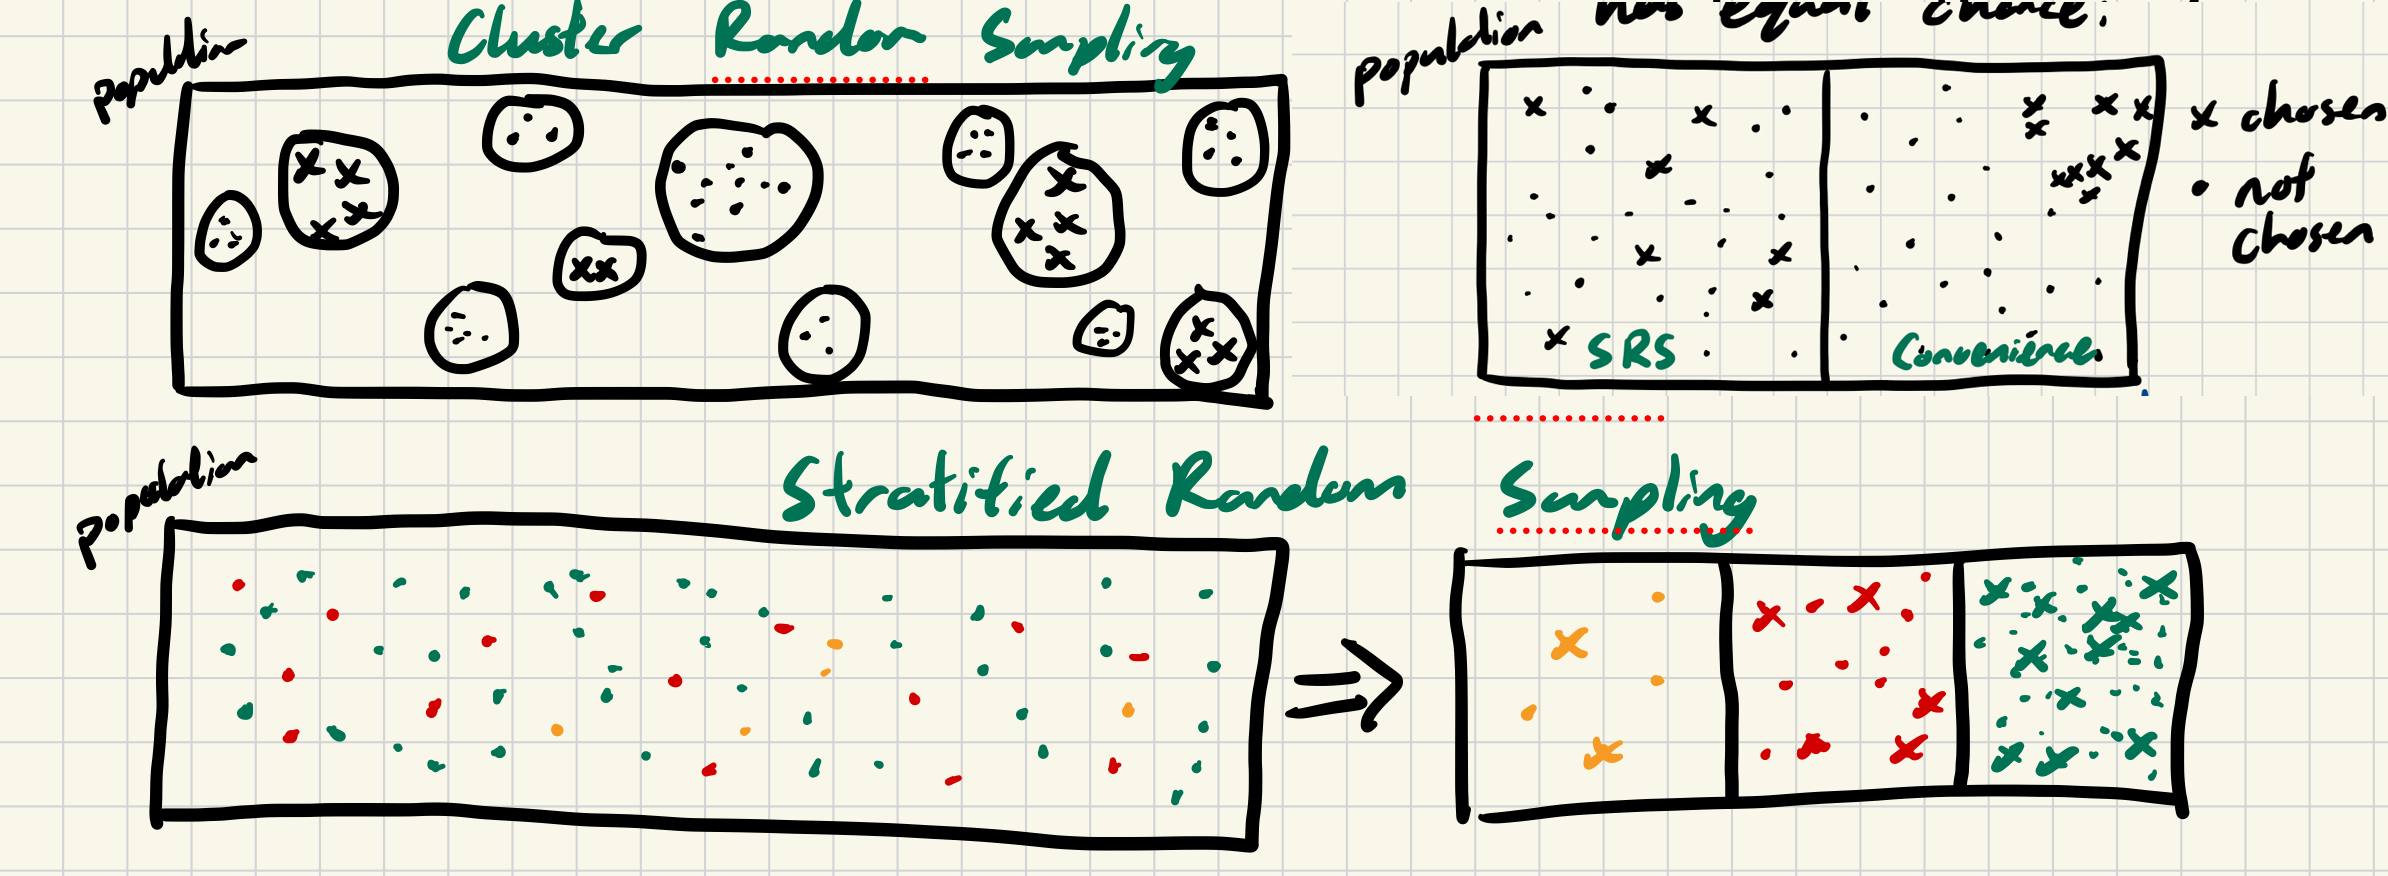
\includegraphics[width=\linewidth]{samplingDesigns.png}
		\end{Figure}
	\item \textcolor{Blue}{Data Collection}
\end{enumerate}
\begin{tabular}{p{0.26\linewidth} p{0.25\linewidth} p{0.26\linewidth}}
	F2F Interview&Phone Interview&Self-Admin Questionnaire\\
	\toprule
	More likely to participate&Less patient, likely to hang up&Lower participation rates\\
	\midrule
	High costs&Low costs&Low costs\\
	\midrule
	May not answer sensitive questions on opinion and lifestyle&&More willing to answer sensitive questions\\
	\bottomrule
\end{tabular}
\textbf{Sampling Bias}: Bias during sampling
\begin{itemize}
	\item Non-Random Sampling
	\item Undercoverage: Non-representative sampling frame\\
		\textcolor{Blue}{eg. Survey through landlines not reaching homeless people}
\end{itemize}
\textbf{Non-Sampling Bias}: Bias during data collection
\begin{itemize}
	\item Nonresponse Bias
		\begin{itemize}
			\item Sampled subjects cannot be reached/refuse to participate
			\item Missing data for certain questions
		\end{itemize}
	\item Response Bias
		\begin{itemize}
			\item Non-honest responses
			\item Confusing/Leading questions
			\item Answering wrongly
		\end{itemize}
\end{itemize}
\paragraph{Experimental Studies}
\begin{itemize}
	\item More sure of a causal relationship as lurking variables' impacts more easily addressed.
	\item Random selection of treatments $\Rightarrow$ Reduced potential for lurking variables.
\end{itemize}
\paragraph{Conducting an Experiment}
\begin{enumerate}
	\item Obtaining experimental units\\
		Typically have to be a convenience sample\\
		$\Rightarrow$\textcolor{Bittersweet}{Representative?}
	\item Assigning to treatments\\
		\textcolor{Blue}{The Control Group}: Placebo/Existing treatments for ethical or comparison reasons\\
		\textcolor{Blue}{Random Assignment}:
		\begin{itemize}
			\item Prevent bias with systematically different non-randomly assigned groups\\
			\item Balance groups on lurking variables to prevent effects on association
		\end{itemize}
	\item Performing Treatment\\
		\textcolor{Blue}{Blinding}: Units unaware of treatment\\
		\textcolor{Blue}{Double-Blinding}: Those in contact with units unaware of treatment
\end{enumerate}

	\section{Probability}
\paragraph{Definitions:}
\begin{itemize}
	\item Probability: Proportion of an outcome in the long run \textcolor{Gray}{(Converges due to law of large numbers)}
	\item Sample Space: Set of ALL possible outcomes
	\item Event: A particular outcome, OR Set of possible outcomes (event $\subseteq$ Sample space)\\
		$P(Event)=\sum P(Outcome)$
	\item Disjoint Events $A,B\iff A\cap B = \varnothing$
	\item Independent Events $A,B$
		\begin{align*}
			&P(A\cap B)&=P(A)\times P(B)\\
			&P(A|B)&=P(A)\\
			&P(B|A)&=P(B)
		\end{align*}
\paragraph{Probability Cheatsheet}
\begin{align*}
	P(A\cup B)&=P(A)+P(B)\\
			  &\quad-P(A\cap B)\\
			  &=P(A)+P(B) \textup{(Disjoint)}\\
	P(A\cap B)&=P(A)\times P(B|A)\\
			  &=P(B)\times P(A|B)\\
			  &=P(A)\times P(B)\textup{(Independent)}\\
	P(A\cap B\cap C)&=P(A)+P(B)+P(C)\\
					&\quad-P(A\cap B)-P(A\cap C)\\
					&\quad-P(B\cap C)-\\
					&\quad P(A\cap B\cap C)\\
	P(A|B)&=\frac{P(A\cap B)}{P(B)}\\
		  &=P(A)\times \frac{P(B|A)}{P(B)}
\end{align*}
For $B_i,B_2,...,B_n$ partitioning S\\
\begin{align*}
	P(A)&=\sum_{i=1}^nP(A\cap B_i)\\
	    &=\sum_{i=1}^n\{P(A|B_i)P(B_i)\}
\end{align*}
\begin{Figure}
	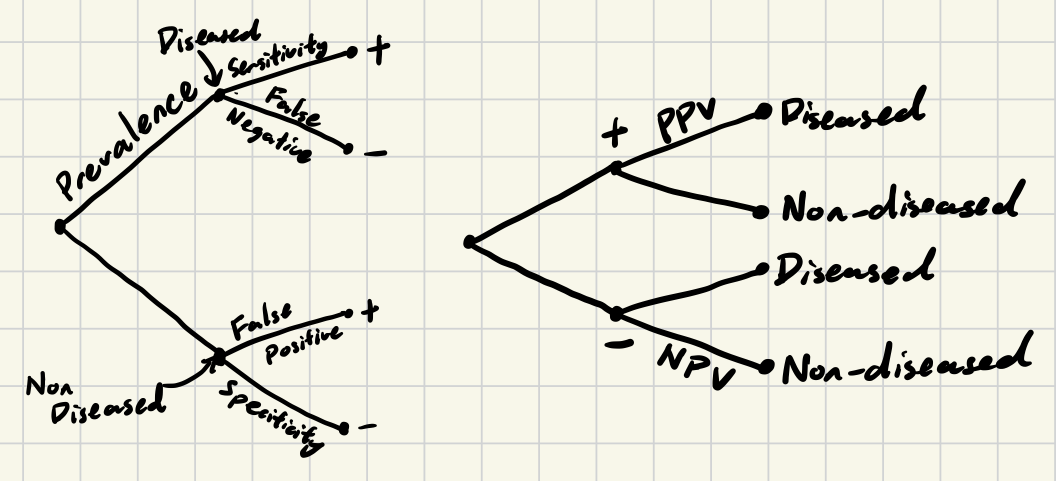
\includegraphics[width=0.893\linewidth]{diseaseProbabilities.png}
\end{Figure}
\end{itemize}
	\section{Distributions}
\paragraph{Mean and Variance of Random Variable $X$}
\textcolor{Blue}{Discrete:}\\
$E(X)=\mu_X=\sum xP(X=x)$\\
$Var(X)=\sum(x-\mu)^2P(X=x)$\\
\textcolor{Blue}{Continuous:}\\
$E(X)=\mu_X=\int xP(X=x)dx$\\
$Var(X)=\int(x-\mu)^2P(X=x)dx$\\
Expected Value $E(X)$:\\
Average in a long run of observations, \textcolor{Bittersweet}{NOT} the expected
value of a single observation!\\
\textbf{Normal Distribution}
\[Norm(\mu,\sigma^2)\qquad \mu\in\mathbb{R},\sigma\in\mathbb{R}^+\]
\begin{enumerate}
	\item Symmetric
	\item Bell-shaped\\
		$0.68$ in $(\mu-\sigma,\mu+\sigma)$\\
		$0.95$ in $(\mu-2\sigma,\mu+2\sigma)$\\
		$0.997$ in $(\mu-3\sigma,\mu+3\sigma)$\\
	\item Approximates many discrete distributions (with large n)
\end{enumerate}
$Z-Score=\frac{x-\mu}{\sigma}$ (No. of standard deviations a value falls from the mean)
Standard Normal: $Norm(0,1)$\\
\textbf{Binomial Distribution}\\
Let $X=$ no. of successes in $n$ trials.
\[X\sim Binom(n, p)\qquad n\in\mathbb{N},p\in[0,1]\]
\begin{enumerate}
	\item Binary Outcomes
	\item Independent $n$ trials\\
		If sampling without replacement,\\
		$n<10\%$ of Population
	\item $P(success)=p$ is a constant\\
		\textcolor{Gray}{Binomial is perfectly symmetric $\iff p=0.5$}
\end{enumerate}
For $x\in\mathbb{N}_{\le n}$,
\[P(X=x)=\frac{n!}{x!(n-x)!}p^x(1-p)^{n-x}\]
\[E(X)=np\qquad Var(X)=np(1-p)\]
\textcolor{Blue}{Approximation by Normal Distribution}\\
$np(1-p)\ge5\vee(np\ge15\wedge n(1-p)\ge15)$\\
$\Rightarrow X\rsimdots Norm(np, np(1-p))$
	\section{Sampling Distribution}
\textcolor{OliveGreen}{Probability distribution that specifies probabilities for the possible values of the statistic}
\begin{tabular}{p{0.2\linewidth} p{0.2\linewidth} p{0.4\linewidth}}
	Population&Data&Sampling\\
	\toprule
	Where a sample comes from&is THE sample&Describes how a sample is likely to look like\\
\end{tabular}
\paragraph{Categorical}
\begin{center}
	Population: proportion \textcolor{Blue}{$p$}\\
	$\Downarrow$\\
	Sample: $n$ observations with proportion \textcolor{Blue}{$\hat{p}$}
\end{center}
Sampling Distribution:
\[successes\sim Binom(n,p)\quad\hat{p}=\frac{successes}{n}\]
$\therefore\mu_{\hat{p}}=p\quad s_{\hat{p}}=\sqrt{\frac{p(1-p)}{n}}$
\textcolor{Blue}{$np(1-p)\ge5\Rightarrow\hat{p}\rsimdots Norm(p,\frac{p(1-p)}{n})$}
\paragraph{Quantitative}
\begin{center}
	Population:\\
	Mean \textcolor{Blue}{$\mu$}, Standard deviation: \textcolor{Blue}{$\sigma$}\\
	$\Downarrow$\\
	Sample $\rsimdots$ Distribution of Population:\\
	$n$ observations with mean \textcolor{Blue}{$\overline{X}$},\\
	Standard deviation: \textcolor{Blue}{$s_X$}
\end{center}
Sampling Distribution:
\[\mu_{\overline{X}}=\mu\quad s_{\overline{X}}=\frac{\sigma}{\sqrt{n}}\]
\textcolor{Bittersweet}{Central Limit Theorem}
\textcolor{Blue}{$n>30\vee pop\sim Norm(\mu,\sigma^2)$\\
$\Rightarrow\overline{X}\sim Norm(\mu,\frac{\sigma^2}{n})$}
	\section{Confidence Intervals}
Getting from Sample Dist. to Parameters: Estimations
\paragraph{Point Estimate}
Ideal Properties:
\begin{itemize}
	\item Unbiased (Centred at parameter)
	\item Small Standard Deviation ($\therefore$ Sample Mean over Median)
\end{itemize}
\paragraph{Confidence Interval}
\begin{itemize}
	\item Indicates precision
	\item Interval around the point estimate (Margin of Error)
	\item Associated with certain degree of confidence ($\approx0.95$)\\
		The probability that it contains $p$
\end{itemize}
If we generated a $(1-\alpha)$ interval using the same method over many random
samples, to estimate many population parameters, in the long run, $(1-\alpha)$ of
those intervals will contain the population parameter.
\paragraph{Confidence Interval: Proportions}
\textcolor{Bittersweet}{Assumptions}:
\begin{itemize}
	\item Data obtained by randomisation
	\item Distribution is $\rsimdots$ Normal ($np(1-p)\ge5$)\\
		For Binomial $\approx$ Normal, $s_{\hat{p}}\approx se$ approximation,
\end{itemize}
$(1-\alpha)$ Confidence Interval:
\begin{align*}
	\hat{p}\pm &\underbrace{q_{1-\frac{\alpha}{2}}(se)}\quad\textcolor{Bittersweet}{s_{\hat{p}}\approx se}=\sqrt{\frac{\hat{p}(1-\hat{p})}{n}}\\
	&\text{Margin of Error}
\end{align*}
\[\textcolor{Blue}{\textup{Margin of Error} \le W}\iff n\ge\frac{q_{1-\frac{\alpha}{2}}^2}{W^2}\hat{p}(1-\hat{p})\]
\begin{align*}
	n \Uparrow&\Rightarrow MoE\Downarrow\\
	(1-\alpha)\Uparrow&\Rightarrow MoE\Uparrow\\
	p\Uparrow&\Rightarrow \hat{p}\Uparrow\Rightarrow MoE\Uparrow
\end{align*}
$n$ ultimately depends on costs and limitations. Rectify:\\
If $p\approx0\vee p\approx1, +2 successes, +2 failures$
\paragraph{Confidence Interval: Mean}
\textcolor{Bittersweet}{Assumptions}:
\begin{itemize}
	\item Data obtained by randomisation
	\item Population Distribution $\rsimdots$ Normal\\
		Robust, but not to \textcolor{Bittersweet}{outliers}:
		\begin{itemize}
			\item Summary statistics $\overline{X}$ and $s_X$ sensitive to outliers.
			\item $\overline{X}$ no longer $\approx\mu_{\overline{X}}=\mu$
		\end{itemize}
\end{itemize}
\textcolor{OliveGreen}{Robustness}
Confidence Interval is robust wrt. the normality assumption
$\Rightarrow$ Performs adequately even when assumption is \textcolor{Bittersweet}{modestly} violated\\
$(1-\alpha)$ Confidence Interval:
\begin{align*}
	\overline{X}\pm&\underbrace{t_{df=n-1,1-\frac{\alpha}{2}}(se)}\quad s_{\overline{X}}\approx se=\frac{s_X}{\sqrt{n}}\\
	&\quad\text{Margin of Error}
\end{align*}
\textcolor{Gray}{$s_X$ is a point estimator of $\sigma$.}\\
For $df\ge30$ ($n>30$), and $\mu\pm3\sigma\approx Range(X)$
\[\textcolor{Blue}{\textup{Margin of Error} \le W}\iff n\ge\frac{\sigma^2q_{1-\frac{\alpha}{2}^2}}{W^2}\]
\begin{align*}
	n \Uparrow&\Rightarrow MoE\Downarrow\\
	(1-\alpha)\Uparrow&\Rightarrow MoE\Uparrow\\
	\sigma^2\Uparrow&\Rightarrow s^2\Uparrow\Rightarrow MoE\Uparrow
\end{align*}
\paragraph{t-Distribution}
Distribution to allow generalisation for small sample sizes but assumes normal distribution
\[t_{df}\qquad df\in\mathbb{R}\]
\[lim_{df\to\infty}t_{df}=Norm(0,1)\]
\[t_{df=30}\approx Norm(0,1)\]
\begin{enumerate}
	\item Bell-shaped
	\item Slightly thicker tails than normal
	\item Shows more variability than normal
\end{enumerate}
	\section{Significance Tests}
\begin{center}
\textbf{Assumptions}\\
Certain conditions or assumptions that the test requires, or makes
$\Downarrow$\\
\textbf{Hypotheses}\\
$H_0$: statement that the parameter takes a particular value (Usually no effect)\\
$H_a$: statement that the parameter falls in some alternative range of values. (Usually represents an effect)\\
\begin{itemize}
	\item Assumed to be true until sufficient evidence against the hypothesis
	\item One/two-sided test ($>$ or $<$ or $\neq$)
\end{itemize}
$\Downarrow$\\
\textbf{Test Statistic}\\
How far the point estimate of the parameter falls from the $H_0$ value, usually in no. of $se$\\
Is a random variable, each sample is an observation\\
Distribution under $H_0$ is the \textcolor{Blue}{null distribution}\\
\textbf{P-Value}\\
Probability that the test statistic equals, or is more extreme, than the observed. Calculated by assuming $H_0$.\\
Smaller P-Value $\Rightarrow$ Stronger evidence against $H_0$\\
$\Downarrow$\\
\textbf{Conclusion}\\
Interpretation of the P-Value, and in context
\end{center}
\textcolor{Blue}{Significance level $\alpha$}: the number such that we reject $H_0$ if the P-Value $\le$\\
\textcolor{Blue}{Statistically Significant}: The results are statistically significant, if the data provides sufficient evidence to reject $H_0$ and support $H_a$
\paragraph{Types of Errors}
\begin{tabular}{c c c}
	&\multicolumn{2}{c}{Decision}\\
	\cmidrule{2-3}
	Reality&Do not reject $H_0$&Reject $H_0$\\
	\midrule
	$H_0$&Correct Conclusion&Type I Error\\
	$H_a$&Type II Error&Correct Conclusion\\
\end{tabular}
\textcolor{Bittersweet}{P(Type I Error)}: Significance level $\alpha$\\
\textcolor{Bittersweet}{P(Type II Error)}: Complex, but inversely related to P(Type I Error). For fixed $\alpha$, prob. decreases:
\begin{itemize}
	\item as parameter moves further into $H_a$, away from $H_0$
	\item as sample size increases
\end{itemize}
Plot: Probability against $p_0$ for fixed $\alpha, n$\\
Power of a test$=1-P(\text{Type II Error})$
\paragraph{Misinterpretations}
\begin{itemize}
	\item "Do not reject $H_0$"$\neq$ \dq Accept $H_0$"\\
	\item Small P-Value does not imply confidence interval is far
\end{itemize}
\paragraph{Significance Test for p}
\textcolor{Bittersweet}{Assumptions}
\begin{itemize}
	\item Categorical Variable
	\item Data obtained using randomisation
	\item Sample size is sufficiently large ($np(1-p)\ge5$)
		Sample size is small $\Rightarrow$ two-sided test is robust.\\Otherwise null-dist$=Binom(n,p_0)$
\end{itemize}
\textcolor{Blue}{Hypotheses}:
\[H_0:p=p_0\quad H_a:p\neq p_0, p>P_0, p<p_0\]
\textcolor{Blue}{Test Statistic}:\\
$z-score_{\hat{p}}$ supposing $H_0$
\[z=\frac{\hat{p}-p_0}{\sqrt{\frac{p_0(1-p_0)}{n}}}\]
\textcolor{Blue}{P-Value}:\\
Null Distribution: $Norm(0,1)$
\[	P-Value=\begin{cases}
	P(Z<z)&left\text{-}sided\\
	P(Z>z)&right\text{-}sided\\
	2\times P(Z>z)&two\text{-}sided
	\end{cases}
\]
\textcolor{Blue}{Conclusion}:
If P-Value is $>\alpha$, strong evidence against $H_0$. Otherwise, we do not have strong evidence against $H_0$.
\paragraph{Significance test for $\overline{X}$}
\dq One Sample t-Test"\\
\textcolor{Bittersweet}{Assumptions}
\begin{itemize}
	\item Quantitative Variable
	\item Data obtained using randomisation
	\item Population distribution $\approx$ Normal\\
		Two-sided test is robust (because CLT)\\
		Except when $n$ is small and $H_a$ is one-sided, sampling distribution is no longer $t$ dist.
\end{itemize}
\textcolor{Blue}{Hypotheses}
\[H_0:\mu=\mu_0\quad H_a:\mu\neq \mu_0, \mu>\mu_0, \mu<\mu_0\]
\textcolor{Blue}{Test Statistic}
$T-Score_{\overline{X}}$ supposing $H_0$
\[T=\frac{\overline{X}-\mu_0}{\frac{s}{\sqrt{n}}}\]
\textcolor{Blue}{P-Value}:\\
Null Distribution: $t_{df=n-1}$
\[ P\text{-}Value=\begin{cases}
	P(t_{df}<T)&left\text{-}sided\\
	P(t_{df}>T)&right\text{-}sided\\
	2\times P(t_{df}>T)&two\text{-}sided\\
\end{cases}
\]
\textcolor{Blue}{Conclusion}
If P-Value is $>\alpha$, strong evidence against $H_0$. Otherwise, we do not have strong evidence against $H_0$.
\paragraph{Two-sided Test vs. Confidence Interval}
$\text{Two-sided test P-Value}\le \alpha\iff(1-\alpha)\text{ Conf-Int does not contain }H_0\text{ value}$
	\section{Bivariate Inference Methods}
\paragraph{Sampling Distribution of $(p_1-p_2)$}
$\mu_{\hat{p_1}-\hat{p_2}}=p_1-p_2$\\
$s_{\hat{p_1}-\hat{p_2}}=\sqrt{\frac{p_1(1-p_1)}{n_1}+\frac{p_2(1-p_2)}{n_2}}$\\
\paragraph{Confidence Interval for $(p_1-p_2)$}
\textcolor{Bittersweet}{Assumptions}
\begin{itemize}
	\item Categorical Response variable observed 
	\item Independent random samples for the two groups
	\item Large sample sizes, $np>10\wedge n(1-p)>10$ for each group
\end{itemize}
$(1-\alpha)$ Confidence Interval:
\[\hat{p_1}-\hat{p_2}\pm q_{1-\frac{\alpha}{2}}(se)\]
\[se=\sqrt{\frac{\hat{p_1}(1-\hat{p_1})}{n_1}+\frac{\hat{p_2}(1-\hat{p_2})}{n_2}}\]\\
If confidence interval contains 0, it is plausible that $(p_1-p_2)=0$, and the proportions might be equal.\\
Sign of values: $p_1>p_2\text{ or }p_1<p_2$\\
Magnitude of values: The size of the true difference in proportions
\paragraph{Significance Test for $(p_1-p_2)$}
Same \textcolor{Bittersweet}{assumptions} as confidence interval\\
\textcolor{Blue}{Hypotheses}
\[H_0\colon p_1=p_2,H_a:p_1\neq p_2, p_1>p_2, p_1<p_2\]
\textcolor{Blue}{Test Statistic}, $\hat{p}$ is the pooled estimate
\[z=\frac{(\hat{p_1}-\hat{p_2})-0}{se_0},se_0=\sqrt{\hat{p}(1-\hat{p})(\frac{1}{n_1}+\frac{1}{n_2})}\]
\textcolor{Blue}{P-Value}\\
Null Distribution: $Norm(0,1)$\\
\textcolor{Blue}{Conclusion}
Groups are (statistically) significantly different if P-Value is small
\paragraph{Sampling Distribution of $(\mu_1-\mu_2)$}
$\mu_{\overline{X_1}-\overline{X_2}}=\mu_1-\mu_2\quad s_{\overline{X_1}-\overline{X_2}}=\sqrt{\frac{\sigma_1^2}{n_1}+\frac{\sigma_2^2}{n_2}}$
Null Distribution: $t_{df}$. $df$ is complex.
\paragraph{Confidence Interval for $(\mu_1-\mu_2)$}
\textcolor{Bittersweet}{Assumptions}
\begin{itemize}
	\item Quantitative response variable observed 
	\item Independent random samples for the two groups
	\item Approximately normal population dist. for each group\\
		Robust, except to outliers [Confidence Interval: Mean]
\end{itemize}
$(1-\alpha)$ Confidence Interval:
\[(\overline{X_1}-\overline{X_2})\pm t_{df,1-\frac{\alpha}{2}}(se),se=\sqrt{\frac{s_1^2}{n_1}+\frac{s_1^2}{n_2}}\]
\paragraph{Significance Test for $(\mu_1-\mu_2)$}
Same \textcolor{Bittersweet}{assumptions} as confidence interval\\
\textcolor{Blue}{Hypotheses}
\[H_0\colon \mu_1=\mu_2,H_a:\mu_1\neq \mu_2\mu_1>\mu_2\mu_1<\mu_2\]
\textcolor{Blue}{Test Statistic}, $se$ same as confidence interval
\[t=\frac{(\overline{X_1}-\overline{X_2})-0}{se_0}\]
\textcolor{Blue}{P-Value} Null Distribution: $t_{df}$\\
\textcolor{Blue}{Conclusion}
Groups are (statistically) significantly different if P-Value is small
\paragraph{Significance Test for $(\mu_1-\mu_2)$, $\sigma_1=\sigma_2$}
$F$ test for comparing standard deviation: P-Value$<\alpha=0.05$\\
$\Uparrow$ NOT robust to population normality assumption\\
\textcolor{Blue}{Assumptions, Test Statistic, P-Value, Conclusion} are all the
same as for non-equal std. dev, but with:
\[se=s_p\sqrt{\frac{1}{n_1}+\frac{1}{n_2}}\]
\[s_p=\sqrt{\frac{(n_1-1)s_1^2+(n_2-1)s_2^2}{x_1+n_2-2}}\]
$df=n_1+n_2-2$
	\section{Linear Regression}
\[Y=\overline{Y}-b(\overline{X})+R(\frac{s_Y}{s_X})X+\epsilon\]
\textcolor{OliveGreen}{Y-intercept} $\overline{Y}-b\overline{X}$\\
Predicted value of $y$ when $x=0$, Might have no interpretative value (if no
observations near x=0).\\
\textcolor{OliveGreen}{Slope} $R(\frac{s_Y}{s_X})$\\
Same sign as R. Amount that $\hat{y}$ changes with one unit increase of $x$
$R^2$ is the \% of variability in the response variable that can be explained by
the linear relationship with the explanatory variable.\\
\textcolor{OliveGreen}{Error term} $\epsilon$\\
\textcolor{Bittersweet}{Assumptions}
\begin{itemize}
	\item Data obtained by randomisation
	\item Relationship between X and Y is linear
	\item Error term $\epsilon\sim Norm(0,\sigma^2)$ where $\sigma$ is a constant
\end{itemize}
\paragraph{Implications of Assumptions}
$\forall X(Y\sim Norm(\beta_0+\beta_1X,\sigma^2))$\\
\paragraph{Ordinary Least Squares Estimation}
Best fit regression is the minimalisation of $\sum_{i=0}^{n-1}e_i^2$\\
\paragraph{Interpreting Info of Linear Regression Models}
$\hat{Y}=\hat{B_0}-\hat{B_1}X$\\
\textcolor{Blue}{Residuals}\\
Quartiles of the residuals of each point with the model
\textcolor{Blue}{Estimate} $\hat{\beta_i}$\\
$\Rightarrow$ Point Estimates of each coefficient in the model\\
\textcolor{Blue}{Std. Error}\\
Standard error of each coefficient. Can be used to obtain a confidence interval\\
\textcolor{Blue}{Residual Standard Error}\\
The standard error of $\hat{\sigma}$
For each point $x_i$, $e_i=y_i-\hat{y_i}$
\begin{itemize}
	\item Could be normalised, to get standard residuals $SR\sim Norm(0,1)$
	\item $\sigma$ is the measure of how far the observations can deviate from best-fit line
\end{itemize}
$\sigma^2$ is the measure of how far the observations can deviate from the best-fit line\\
\textcolor{Blue}{Multiple R-squared}\\
Coefficient of Determination of linear model
\paragraph{Hypothesis Testing on Linear Models}
\textbf{t-Test}\\
The significance of one regressor.\\
\textcolor{Bittersweet}{Assumptions} Same as assumptions of model\\
\textcolor{Blue}{Hypothesis}
$H_0\colon\beta_i=0\text{ OR Regressor }i\text{ is NOT sigificant}$\\
$H_a\colon\beta_i\neq0\text{ OR Regressor }i\text{ is significant}$\\
\textcolor{Blue}{Test Statistic}
\[t=\frac{\hat{B_i}}{se}\]
\textcolor{Blue}{P-Value}\\
Null-Distribution: $t$ Distribution, $df=n-$no. of coefficients\\
\textcolor{Blue}{Conclusion}\\
The coefficient is (not) significantly different from 0 at $\alpha$-level\\
\textbf{F-test}\\
\textcolor{Bittersweet}{Assumptions} Same as assumptions of model\\
\textcolor{Blue}{Hypothesis}\\
$H_0\colon$ model is NOT significant OR all the coefficients except $\beta_0$ are zero\\
$H_a\colon$ model is significant OR at least one of the coefficients except $\beta_0$ are non-zero\\
\textcolor{Blue}{Test Statistic} F-statistic from R output\\
$F=t^2$ for Simple Linear Regression\\
\textcolor{Blue}{P-Value}\\
Null-Distribution: $F$ Distribution,\\
$df1=$no. of coefficients$-1$\\
$df2=n-$no. of coefficients\\
Find right-sided P-Value on $F$ Distribution\\
\textcolor{Blue}{Conclusion}\\
The data provides (in)sufficient evidence that the built model is significant.\\
$P-Value<\alpha\Rightarrow$ ALL regressors used in the model are not significant, $Y=\beta_0$
\paragraph{Checking Assumptions of Linear Model}
Before fitting model, scatterplot of Y against X:
\begin{enumerate}
	\item Linearity (No curved bands)
	\item Constant Variance (Funnel shape)
\end{enumerate}
To verify the assumption $\epsilon\sim Norm(0,\sigma^2)$
\begin{enumerate}
	\item SR against $\hat{Y_i}$
	\item SR against $X$\\
		Points scatter randomly around 0, within $(-3, 3)$
		Funnel shaped observed $\Rightarrow$ Constant variance assumption violated
	\item Histogram of SR
	\item QQ Plot of SR\\
		SR has a normal distribution
		Skewed Distribution $\Rightarrow$ Normality assumption violated
\end{enumerate}
Possible Fixes
\begin{itemize}
	\item Add higher order terms
	\item Transform response into $\ln(Y),\sqrt{Y},\frac{1}{Y}$
	\item Add more regressors
	\item Non-linear model required
\end{itemize}
$\left|SR\right|>3\Rightarrow$Potential outlier\\
Cook's Distance$>1\Rightarrow$Potential influential point\\
Avoid Extrapolation (Estimation using regressors outside domain)
\paragraph{Coefficient of Determination}
\textcolor{Blue}{Interpretation}:\\
The proportion of total variation of the response (of sample mean
$\overline{Y}$) that is explained by the model.\\
For simple model: $\sqrt{R^2}=\left|Cor(X,Y)\right|$\\
$R^2=1\Rightarrow\forall i(\hat{Y_i}=Y_i)$
Adding regressors will always increase, or not change $R^2$. Use adjusted $R^2$
\[R_{adj}^2=1-\frac{(1-R^2)(n-1)}{n-\text{no. of coefficients}}\]
\paragraph{Indicator Variables}
Each indicator splits the model into two equations, on whether the indicator is $1$ or $0$\\
$n$ categories require $n-1$ indicators\\
Identify the reference category when every indicator is $0$.
Use anova P-Value for significance of categorical variables
\end{multicols*}
\end{document}